% ថ្នាក់ទី ១១ (វិទ្យាសាស្ត្រ) · ជំពូកទី ២ · មេរៀនទី ១ · សៀវភៅទំព័រ ៥៧–៧១
\chapter{អនុគមន៍អិចស្ប៉ូណង់ស្យែល}

នៅក្នុងជំពូកនេះ គេចាប់ផ្តើមសិក្សាពីបញ្ញត្តិនៃអនុគមន៍អិចស្ប៉ូណង់ស្យែល សង់ក្រាបតាងអនុគមន៍ ដោះស្រាយសមីការ និងវិសមីការអិចស្ប៉ូណង់ស្យែល ដែលជាមធ្យោបាយសំខាន់សម្រាប់សិក្សាពីបញ្ញត្តិ ក្រាប សមីការ និងវិសមីការលោការីត ។ បន្ទាប់ពីទទួលបានបញ្ញត្តិអនុគមន៍អិចស្ប៉ូណង់ស្យែលនិងលោការីត សិស្សអាចយកចំណេះដឹងនិងបំណិនទៅដោះស្រាយចំណោទបញ្ហាដែលទាក់ទងនឹងការប្រាក់ កំណើនភ្ញៀវទេសចរដែលចូលមកទស្សនាប្រាសាទអង្គរវត្ត កំណើនប្រជាជន និងសម្រាប់ដោះស្រាយចំណោទបញ្ហាផ្សេងទៀតដែលជួបប្រទះក្នុងជីវភាពប្រចាំថ្ងៃ ។

\begin{objBox}[វត្ថុបំណង]
\begin{enumerate}[1]
  \item សង់ក្រាបនៃអនុគមន៍អិចស្ប៉ូណង់ស្យែល
  \item ដោះស្រាយសមីការនិងវិសមីការអិចស្ប៉ូណង់ស្យែល ។
\end{enumerate}
\end{objBox}

\section{អនុគមន៍អិចស្ប៉ូណង់ស្យែល}

\subsection{និយមន័យនៃអិចស្ប៉ូណង់ស្យែល}

\begin{example}[ឧទាហរណ៍]
គេឱ្យកន្សោមស្វ័យគុណដូចខាងក្រោម ៖
\begin{enumerate}[a]
  \item $(-3)^x$, $1^x$, $0^x$
  \item $3^x$ ហៅថា \textbf{អិចស្ប៉ូណង់ស្យែល} ។
  \item $\left(\dfrac{1}{3}\right)^{2x+1}$ ហៅថា \textbf{អិចស្ប៉ូណង់ស្យែល} ។
\end{enumerate}
\end{example}

\begin{definition}
អិចស្ប៉ូណង់ស្យែលគឺជាកន្សោមស្វ័យគុណដែលមាននិទស្សន្តជាអថេរ និងមានគោលជាចំនួនវិជ្ជមានខុសពី $1$ ។
\end{definition}

\subsection{និយមន័យនៃអនុគមន៍អិចស្ប៉ូណង់ស្យែល}

\begin{example}[ឧទាហរណ៍]
គេឱ្យទំនាក់ទំនងដូចខាងក្រោម ៖
\begin{enumerate}[a]
  \item $f(x) = (-3)^x$
  \item $f(x) = 1^x$
  \item $f(x) = 0^x$
  \item $f(x) = 3^x$ ទំនាក់ទំនងនេះហៅថា \textbf{អនុគមន៍អិចស្ប៉ូណង់ស្យែល} ។
  \item $f(x) = 3^{-x+1}$ ទំនាក់ទំនងនេះហៅថា \textbf{អនុគមន៍អិចស្ប៉ូណង់ស្យែល} ។
\end{enumerate}
\end{example}

\begin{definition}
អនុគមន៍អិចស្ប៉ូណង់ស្យែលគឺជាអនុគមន៍ស្វ័យគុណដែលមានអថេរឯករាជ្យជានិទស្សន្ត និងមានគោលជាចំនួនវិជ្ជមានខុសពី $1$ ។
\end{definition}

\subsection{ក្រាបនៃអនុគមន៍អិចស្ប៉ូណង់ស្យែល}

\begin{example}[ឧទាហរណ៍]
គេសង់ក្រាបនៃអនុគមន៍ $f(x) = 2^x$, $g(x) = (1.5)^x$, $h(x) = 1^x$, $k(x) = (0.5)^x$ ក្នុងតម្រុយតែមួយ ។

តារាងតម្លៃត្រូវគ្នានៃ $x$ និង $y$
\[
\begin{array}{|c|c|c|c|c|c|}\hline
x & -2 & -1 & 0 & 1 & 2\\ \hline
y = 1.5^x & 0.44 & 0.66 & 1 & 1.5 & 2.25\\ \hline
\end{array}
\]
\begin{center}
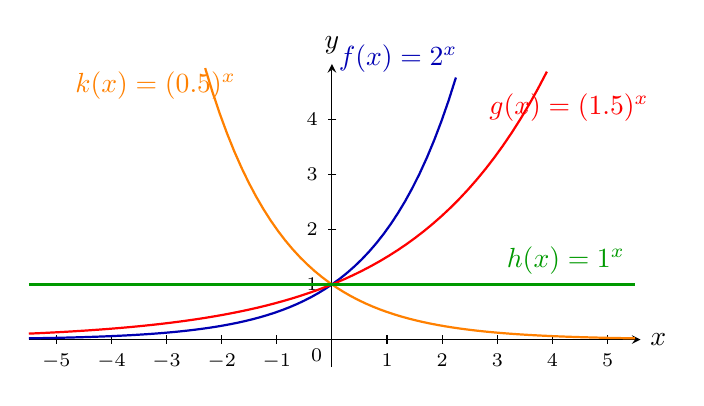
\begin{tikzpicture}[scale=0.7,>=stealth]
  \draw[->] (-5.5,0) -- (5.6,0) node[right] {$x$};
  \draw[->] (0,-0.5) -- (0,5) node[above] {$y$};
  \foreach \x in {-5,-4,-3,-2,-1,1,2,3,4,5} \draw (\x,0.08) -- (\x,-0.08) node[below] {\scriptsize $\x$};
  \foreach \y in {1,2,3,4} \draw (0.08,\y) -- (-0.08,\y) node[left] {\scriptsize $\y$};
  \node[below left] at (0,0) {\scriptsize $0$};
  \draw[thick,orange,domain=-2.3:5.5,samples=60] plot (\x,{0.5^\x});
  \draw[thick,blue!70!black,domain=-5.5:2.25,samples=60] plot (\x,{2^\x});
  \draw[thick,red,domain=-5.5:3.9,samples=60] plot (\x,{1.5^\x});
  \draw[thick,green!60!black] (-5.5,1) -- (5.5,1) node[above left] {$h(x) = 1^x$};
  \node[orange] at (-3.2,4.6) {$k(x) = (0.5)^x$};
  \node[blue!70!black] at (1.2,5.1) {$f(x) = 2^x$};
  \node[red] at (4.3,4.2) {$g(x) = (1.5)^x$};
\end{tikzpicture}
\end{center}
\end{example}

តាមក្រាបយើងសង្កេតឃើញថា គ្រប់ក្រាបរបស់អនុគមន៍អិចស្ប៉ូណង់ស្យែលដែលមានរាង $y = a^x$ កាត់តាមចំណុចដែលមានកូអរដោនេ $(0, 1)$ ជានិច្ច ។
\begin{itemize}
  \item បើ $x > 0$ នោះ $(1.5)^x < 2^x$ ។ ដូច្នេះ ក្នុងកាដ្រង់ទី $1$ ក្រាបនៃអនុគមន៍ $g(x) = (1.5)^x$ ស្ថិតនៅក្រោមក្រាបនៃអនុគមន៍ $f(x) = 2^x$ ។
  \item អនុគមន៍ $h(x) = 1^x$ មានក្រាបជាបន្ទាត់ស្របនឹងអ័ក្សអាប់ស៊ីស និងនៅពីលើអ័ក្សអាប់ស៊ីសចំនួន $1$ ឯកតា ចំពោះគ្រប់តម្លៃ $x$ ។
  \item បើ $x > 0$ នោះ $(0.5)^x < 1$ ។ ដូច្នេះ បើ $x$ យកតម្លៃកើនធំឡើងៗ នោះ $k(x) = (0.5)^x$ មានតម្លៃចុះតូចទៅៗ ហើយខិតទៅរក $0$ ។
  \item បើ $x < 0$ នោះ $(0.5)^x$ មានតម្លៃធំឡើងៗគ្មានកំណត់ ។
\end{itemize}

\begin{formulaBox}[ជាទូទៅ]
អនុគមន៍អិចស្ប៉ូណង់ស្យែល $y = a^x$ មានក្រាប
\begin{itemize}
  \item បើ $a > 1$ ក្រាបនៃ $y = a^x$ កើនពីឆ្វេងទៅស្តាំ គេថា $y = a^x$ ជាអនុគមន៍កើន
  \item បើ $0 < a < 1$ ក្រាបនៃ $y = a^x$ ចុះពីឆ្វេងទៅស្តាំ គេថា $y = a^x$ ជាអនុគមន៍ចុះ
  \item អនុគមន៍ $y = a^x$ វិជ្ជមានជានិច្ច $\forall x \in \mathbb{R}$ បើ $a$ ជាចំនួនពិតវិជ្ជមាននិងខុសពី $1$
  \item ក្រាបនៃអនុគមន៍ $y = a^x$ កាត់អ័ក្សអរដោនេត្រង់ $(0, 1)$ ជានិច្ច ។
\end{itemize}
\end{formulaBox}

\begin{example}[លំហាត់គំរូ ១]
សង់ក្រាប \quad ក. $y = 4^x$ \qquad ខ. $y = \left(\dfrac{1}{4}\right)^x$ ។
\end{example}
\ans
ក. តារាងតម្លៃត្រូវគ្នានៃ $x$ និង $y$
\[
\begin{array}{|c|c|c|c|c|c|}\hline
x & -2 & -1 & 0 & 1 & 2\\ \hline
y = 4^x & 0.06 & 0.25 & 1 & 4 & 16\\ \hline
\end{array}
\]
\begin{center}
\begin{tikzpicture}[scale=0.7,>=stealth]
  \draw[->] (-4.5,0) -- (5,0) node[right] {$x$};
  \draw[->] (0,-1) -- (0,5.5) node[above] {$y$};
  \draw (-1,0.08) -- (-1,-0.08) node[below] {\scriptsize $-1$};
  \draw (1,0.08) -- (1,-0.08) node[below] {\scriptsize $1$};
  \node[below left] at (0,0) {\scriptsize $0$};
  \node[left] at (0,1) {\scriptsize $1$};
  \node[left] at (0,4) {\scriptsize $4$};
  \draw[dotted] (0,4) -- (1,4) -- (1,0);
  \draw[thick,green!60!black,domain=-4.5:1.2,samples=60] plot (\x,{4^\x});
  \node[green!60!black] at (2,4.8) {$y = 4^x$};
\end{tikzpicture}
\end{center}
ខ. តារាងតម្លៃត្រូវគ្នានៃ $x$ និង $y$
\[
\begin{array}{|c|c|c|c|c|c|}\hline
x & -2 & -1 & 0 & 1 & 2\\ \hline
y = (1/4)^x & 16 & 4 & 1 & 0.25 & 0.06\\ \hline
\end{array}
\]
\begin{center}
\begin{tikzpicture}[scale=0.7,>=stealth]
  \draw[->] (-5,0) -- (4.5,0) node[right] {$x$};
  \draw[->] (0,-1) -- (0,5.5) node[above] {$y$};
  \draw (-1,0.08) -- (-1,-0.08) node[below] {\scriptsize $-1$};
  \draw (1,0.08) -- (1,-0.08) node[below] {\scriptsize $1$};
  \node[below left] at (0,0) {\scriptsize $0$};
  \node[right] at (0,1) {\scriptsize $1$};
  \node[right] at (0,4) {\scriptsize $4$};
  \draw[dotted] (0,4) -- (-1,4) -- (-1,0);
  \draw[thick,green!60!black,domain=-1.2:4.5,samples=60] plot (\x,{0.25^\x});
  \node[green!60!black] at (-2.4,4.8) {$y = \left(\frac{1}{4}\right)^x$};
\end{tikzpicture}
\end{center}

\begin{pro}
សង់ក្រាបអនុគមន៍ \quad ក. $y = 10^x$ \qquad ខ. $y = \left(\dfrac{1}{10}\right)^x$ ។
\end{pro}

\subsection{លក្ខណៈក្រាបនៃអនុគមន៍អិចស្ប៉ូណង់ស្យែល}

\begin{example}[ឧទាហរណ៍ ក]
សង់ក្រាបនៃអនុគមន៍ $y = 2^x + 1$ ។

តារាងតម្លៃត្រូវគ្នានៃ $x$ និង $y$
\[
\begin{array}{|c|c|c|c|c|c|}\hline
x & -2 & -1 & 0 & 1 & 2\\ \hline
y = 2^x & 0.25 & 0.50 & 1 & 2 & 4\\ \hline
y = 2^x + 1 & 1.25 & 1.50 & 2 & 3 & 5\\ \hline
\end{array}
\]
\begin{center}
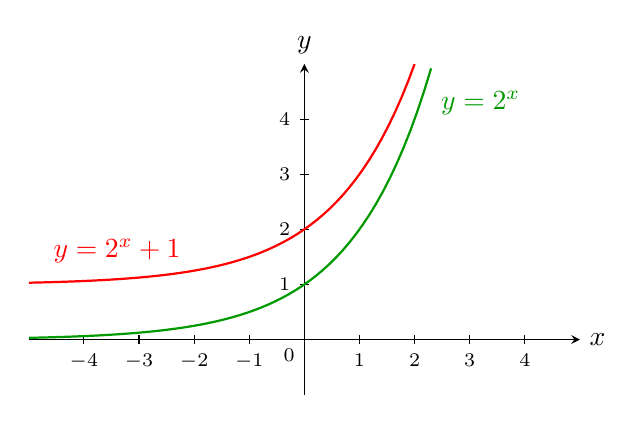
\begin{tikzpicture}[scale=0.7,>=stealth]
  \draw[->] (-5,0) -- (5,0) node[right] {$x$};
  \draw[->] (0,-1) -- (0,5) node[above] {$y$};
  \foreach \x in {-4,-3,-2,-1,1,2,3,4} \draw (\x,0.08) -- (\x,-0.08) node[below] {\scriptsize $\x$};
  \foreach \y in {1,2,3,4} \draw (0.08,\y) -- (-0.08,\y) node[left] {\scriptsize $\y$};
  \node[below left] at (0,0) {\scriptsize $0$};
  \draw[thick,green!60!black,domain=-5:2.3,samples=60] plot (\x,{2^\x});
  \draw[thick,red,domain=-5:2,samples=60] plot (\x,{2^\x+1});
  \node[green!60!black] at (3.2,4.3) {$y = 2^x$};
  \node[red] at (-3.4,1.6) {$y = 2^x + 1$};
\end{tikzpicture}
\end{center}
តាមក្រាបគេសង្កេតឃើញថា ដើម្បីសង់ក្រាប $y = 2^x + 1$ ដំបូងគេសង់ក្រាប $y = 2^x$ រួចរំកិលចំនួនមួយឯកតាឡើងលើស្របអ័ក្ស $(oy)$ គេបានក្រាប $y = 2^x + 1$ ។
\end{example}

\begin{example}[ឧទាហរណ៍ ខ]
សង់ក្រាបនៃអនុគមន៍ $y = 2^{x+1}$ ។

តារាងតម្លៃត្រូវគ្នានៃ $x$ និង $y$
\[
\begin{array}{|c|c|c|c|c|c|}\hline
x & -2 & -1 & 0 & 1 & 2\\ \hline
y = 2^x & 0.25 & 0.50 & 1 & 2 & 4\\ \hline
y = 2^{x+1} & 0.50 & 1 & 2 & 4 & 8\\ \hline
\end{array}
\]
\begin{center}
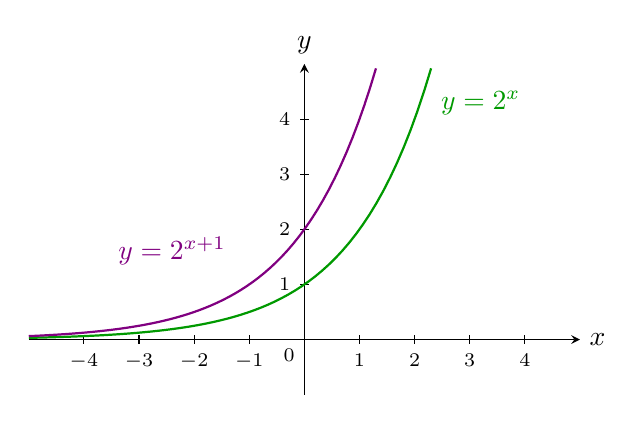
\begin{tikzpicture}[scale=0.7,>=stealth]
  \draw[->] (-5,0) -- (5,0) node[right] {$x$};
  \draw[->] (0,-1) -- (0,5) node[above] {$y$};
  \foreach \x in {-4,-3,-2,-1,1,2,3,4} \draw (\x,0.08) -- (\x,-0.08) node[below] {\scriptsize $\x$};
  \foreach \y in {1,2,3,4} \draw (0.08,\y) -- (-0.08,\y) node[left] {\scriptsize $\y$};
  \node[below left] at (0,0) {\scriptsize $0$};
  \draw[thick,green!60!black,domain=-5:2.3,samples=60] plot (\x,{2^\x});
  \draw[thick,violet,domain=-5:1.3,samples=60] plot (\x,{2^(\x+1)});
  \node[green!60!black] at (3.2,4.3) {$y = 2^x$};
  \node[violet] at (-2.4,1.6) {$y = 2^{x+1}$};
\end{tikzpicture}
\end{center}
តាមក្រាប គេសង្កេតឃើញថា ដើម្បីសង់ក្រាប $y = 2^{x+1}$ ដំបូងគេសង់ក្រាប $y = 2^x$ រួចរំកិលចំនួនមួយឯកតាទៅខាងឆ្វេងស្របអ័ក្ស $(ox)$ គេបានក្រាប $y = 2^{x+1}$ ។
\end{example}

\begin{example}[ឧទាហរណ៍ គ]
សង់ក្រាបនៃអនុគមន៍ $y = 2^{x-2}$ ។

តារាងតម្លៃត្រូវគ្នានៃ $x$ និង $y$
\[
\begin{array}{|c|c|c|c|c|c|}\hline
x & -2 & -1 & 0 & 1 & 2\\ \hline
y = 2^x & 0.25 & 0.50 & 1 & 2 & 4\\ \hline
y = 2^{x-2} & 0.06 & 0.12 & 0.25 & 0.5 & 1\\ \hline
\end{array}
\]
\begin{center}
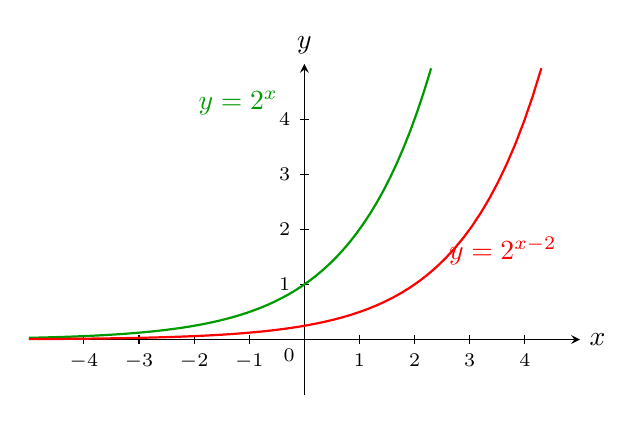
\begin{tikzpicture}[scale=0.7,>=stealth]
  \draw[->] (-5,0) -- (5,0) node[right] {$x$};
  \draw[->] (0,-1) -- (0,5) node[above] {$y$};
  \foreach \x in {-4,-3,-2,-1,1,2,3,4} \draw (\x,0.08) -- (\x,-0.08) node[below] {\scriptsize $\x$};
  \foreach \y in {1,2,3,4} \draw (0.08,\y) -- (-0.08,\y) node[left] {\scriptsize $\y$};
  \node[below left] at (0,0) {\scriptsize $0$};
  \draw[thick,green!60!black,domain=-5:2.3,samples=60] plot (\x,{2^\x});
  \draw[thick,red,domain=-5:4.3,samples=60] plot (\x,{2^(\x-2)});
  \node[green!60!black] at (-1.2,4.3) {$y = 2^x$};
  \node[red] at (3.6,1.6) {$y = 2^{x-2}$};
\end{tikzpicture}
\end{center}
តាមក្រាប គេសង្កេតឃើញថា ដើម្បីសង់ក្រាប $y = 2^{x-2}$ ដំបូងគេសង់ក្រាប $y = 2^x$ រួចរំកិលចំនួនពីរឯកតាទៅខាងស្តាំស្របអ័ក្ស $(ox)$ គេបានក្រាប $y = 2^{x-2}$ ។
\end{example}

\begin{example}[ឧទាហរណ៍ ឃ]
សង់ក្រាបនៃអនុគមន៍ $y = -2^x$ ។

តារាងតម្លៃត្រូវគ្នានៃ $x$ និង $y$
\[
\begin{array}{|c|c|c|c|c|c|}\hline
x & -2 & -1 & 0 & 1 & 2\\ \hline
y = 2^x & 0.25 & 0.50 & 1 & 2 & 4\\ \hline
y = -2^x & -0.25 & -0.50 & -1 & -2 & -4\\ \hline
\end{array}
\]
\begin{center}
\begin{tikzpicture}[scale=0.7,>=stealth]
  \draw[->] (-4.5,0) -- (4.5,0) node[right] {$x$};
  \draw[->] (0,-4.5) -- (0,4) node[above] {$y$};
  \foreach \x in {-3,-2,-1,1,2,3} \draw (\x,0.08) -- (\x,-0.08) node[below] {\scriptsize $\x$};
  \foreach \y in {-4,-3,-2,-1,1,2,3} \draw (0.08,\y) -- (-0.08,\y) node[left] {\scriptsize $\y$};
  \node[below left] at (0,0) {\scriptsize $0$};
  \draw[thick,green!60!black,domain=-4.5:1.9,samples=60] plot (\x,{2^\x});
  \draw[thick,red,domain=-4.5:2.1,samples=60] plot (\x,{-2^\x});
  \node[green!60!black] at (2.8,2.8) {$y = 2^x$};
  \node[red] at (2.8,-2.6) {$y = -2^x$};
\end{tikzpicture}
\end{center}
តាមក្រាប គេសង្កេតឃើញថា ដំបូងគេសង់ក្រាប $y = 2^x$ រួចគូសក្រាបឆ្លុះគ្នាធៀបនឹងអ័ក្ស $(ox)$ គេបានក្រាប $y = -2^x$ ។
\end{example}

\begin{formulaBox}[ជាទូទៅ]
\begin{itemize}
  \item ដើម្បីសង់ក្រាបនៃអនុគមន៍ $y = a^x + q$ គេត្រូវសង់ក្រាប $y = a^x$ រួចធ្វើបម្លែងកិលក្រាបស្របអ័ក្ស $(oy)$ ចំនួន $q$ ឯកតាឡើងលើបើ $q > 0$ ហើយចំនួន $q$ ឯកតាចុះក្រោមបើ $q < 0$ ។
  \item ដើម្បីសង់ក្រាបនៃអនុគមន៍ $y = a^{(x-p)}$ គេត្រូវសង់ក្រាប $y = a^x$ រួចធ្វើបម្លែងកិលក្រាបស្របអ័ក្ស $(ox)$ ចំនួន $p$ ឯកតាទៅខាងស្តាំបើ $p > 0$ ហើយចំនួន $p$ ឯកតាទៅខាងឆ្វេងបើ $p < 0$ ។
  \item ដើម្បីសង់ក្រាបនៃអនុគមន៍ $y = -a^x$ គេត្រូវសង់ក្រាប $y = a^x$ រួចគូសក្រាបឆ្លុះធៀបនឹងអ័ក្ស $(ox)$ គេបានក្រាប $y = -a^x$ ។
\end{itemize}
\end{formulaBox}

\begin{pro}
សង់ក្រាបអនុគមន៍
\begin{tasks}(3)
  \task $y = 3^x - 3$
  \task $y = 3^x + 1$
  \task $y = (1.5)^{x-2}$
  \task $y = (1.5)^{x+3}$
  \task $y = -5^x$ ។
\end{tasks}
\end{pro}

\section{សមីការនិងវិសមីការអិចស្ប៉ូណង់ស្យែល}

\subsection{សមីការអិចស្ប៉ូណង់ស្យែល}

\begin{example}[ឧទាហរណ៍]
គេឱ្យសមភាពដូចខាងក្រោម ៖
\begin{enumerate}[a]
  \item $(-3)^x = -2187$
  \item $1^x = 1$
  \item $0^x = 0$
  \item $3^x = 2187$ សមភាពដែលមាននិទស្សន្តជាអញ្ញាត និងមានគោលជាចំនួនវិជ្ជមានខុសពី $1$ ហៅថា \textbf{សមីការអិចស្ប៉ូណង់ស្យែល} ។
\end{enumerate}
\end{example}

\begin{definition}
សមីការអិចស្ប៉ូណង់ស្យែលគឺជាសមីការស្វ័យគុណដែលមាននិទស្សន្តជាអញ្ញាត និងមានគោលជាចំនួនវិជ្ជមានខុសពី $1$ ។
\end{definition}

\begin{example}[លំហាត់គំរូ ២]
ដោះស្រាយសមីការ
\begin{tasks}(2)
  \task $2^{3x+5} = 128$
  \task $5^{x-3} = \dfrac{1}{25}$
  \task $\left(\dfrac{1}{9}\right)^x = 81^{x+4}$
  \task $49^x = 7^{x^2-15}$
  \task $36^{2x} = 216^{x-1}$
  \task $10^{x-1} = 100^{2x-3}$ ។
\end{tasks}
\end{example}
\ans
\begin{enumerate}[a]
  \item $2^{3x+5} = 128$, \ $2^{3x+5} = 2^7$, \ $3x + 5 = 7$ នាំឱ្យ $x = \dfrac{2}{3}$
  \item $5^{x-3} = \dfrac{1}{25}$, \ $5^{x-3} = 5^{-2}$, \ $x - 3 = -2$ នាំឱ្យ $x = 1$
  \item $\left(\dfrac{1}{9}\right)^x = 81^{x+4}$, \ $9^{-x} = 9^{2(x+4)}$, \ $-x = 2x + 8$ នាំឱ្យ $x = -\dfrac{8}{3}$
  \item $49^x = 7^{x^2-15}$, \ $7^{2x} = 7^{x^2-15}$, \ $2x = x^2 - 15$ នាំឱ្យ $x = 5$, $x = -3$
  \item $36^{2x} = 216^{x-1}$, \ $6^{2(2x)} = 6^{3(x-1)}$, \ $4x = 3x - 3$ នាំឱ្យ $x = -3$
  \item $10^{x-1} = 100^{2x-3}$, \ $10^{x-1} = 10^{2(2x-3)}$, \ $x - 1 = 4x - 6$ នាំឱ្យ $x = \dfrac{5}{3}$ ។
\end{enumerate}

\begin{pro}
\begin{tasks}(2)
  \task $5^x \cdot 2^{\frac{2x-1}{x+1}} = 50$
  \task $3^{4x+8} - 4 \cdot 3^{2x+5} + 27 = 0$
  \task $27^x + 12^x = 2 \cdot 8^x$
  \task $3^{2x^2-6x+3} + 6^{x^2-3x+1} = 2^{2x^2-6x+3}$ ។
\end{tasks}
\ans
\begin{tasks}(2)
  \task $x = 2$, $x = -1 - \log_5 2$
  \task $x = -1$, $x = -\dfrac{3}{2}$
  \task $x = 0$
  \task $x = 1$, $x = 2$ ។
\end{tasks}
\end{pro}

\subsection{វិសមីការអិចស្ប៉ូណង់ស្យែល}

\begin{example}[ឧទាហរណ៍]
ដោះស្រាយវិសមីការ
\begin{enumerate}[a]
  \item $2^x < 2^3$ គេបាន $x < 3$ ជាចម្លើយរបស់វិសមីការព្រោះតម្លៃ $x < 3$ ផ្ទៀងផ្ទាត់ឱ្យវិសមីការ ។
  \item $\left(\dfrac{1}{2}\right)^x < \left(\dfrac{1}{2}\right)^3$ គេបាន $x > 3$ ជាចម្លើយរបស់វិសមីការ ព្រោះតម្លៃ $x > 3$ ផ្ទៀងផ្ទាត់ឱ្យវិសមីការ ។
\end{enumerate}
\end{example}

\begin{formulaBox}[ជាទូទៅ]
វិសមីការអិចស្ប៉ូណង់ស្យែលមានទម្រង់ $a^x > a^y$
\begin{itemize}
  \item បើ $a > 1$ វិសមីការ $a^x > a^y$ សមមូល $x > y$ ហើយវិសមីការ $a^x < a^y$ សមមូល $x < y$ ។
  \item បើ $0 < a < 1$ វិសមីការ $a^x > a^y$ សមមូល $x < y$ ហើយវិសមីការ $a^x < a^y$ សមមូល $x > y$ ។
\end{itemize}
\end{formulaBox}

\begin{example}[លំហាត់គំរូ ៣]
ដោះស្រាយវិសមីការ
\begin{tasks}(3)
  \task $25^{2x} \le 5\sqrt{5}$
  \task $\left(\dfrac{2}{3}\right)^{-3x} > \dfrac{16}{81}$
  \task $5^x > -7$
  \task $(0.1)^x > 10$
  \task $27^x \cdot 3^{1-x} < \dfrac{1}{3}$
  \task $2^{9x-x^3} < 1$
  \task $\left(\dfrac{1}{3}\right)^{\frac{2}{x}} + 3\left(\dfrac{1}{3}\right)^{\frac{1}{x}+1} > 12$ ។
\end{tasks}
\end{example}
\ans
\begin{enumerate}[a]
  \item $25^{2x} \le 5\sqrt{5}$, \ $5^{4x} \le 5^{\frac{3}{2}}$, \ $x \le \dfrac{3}{8}$ ។
  \item $\left(\dfrac{2}{3}\right)^{-3x} > \dfrac{16}{81}$, \ $\left(\dfrac{2}{3}\right)^{-3x} > \left(\dfrac{2}{3}\right)^4$, \ $-3x < 4$, \ $x > -\dfrac{4}{3}$ ។
  \item $5^x > -7$, \ $5^x$ វិជ្ជមានជានិច្ច, $-7$ អវិជ្ជមានជានិច្ច ដូច្នេះ វិសមីការមានចម្លើយចំពោះ $\forall x \in \mathbb{R}$ ។
  \item $(0.1)^x > 10$, \ $10^{-x} > 10$, \ $-x > 1$, \ $x < -1$ ។
  \item $27^x \cdot 3^{1-x} < \dfrac{1}{3}$, \ $3^{3x} \cdot 3^{1-x} < 3^{-1}$, \ $3^{2x+1} < 3^{-1}$, \ $2x + 1 < -1$ ឬ $x < -1$ ។
  \item $2^{9x-x^3} < 1$, \ $2^{9x-x^3} < 2^0$, \ $9x - x^3 < 0$, \ $(9 - x^2)x < 0$, \ $-3 < x < 0$ ឬ $x > 3$ ។
  \item $\left(\dfrac{1}{3}\right)^{\frac{2}{x}} + 3\left(\dfrac{1}{3}\right)^{\frac{1}{x}+1} > 12$, \ $\left[\left(\dfrac{1}{3}\right)^{\frac{1}{x}}\right]^2 + \left(\dfrac{1}{3}\right)^{\frac{1}{x}} - 12 > 0$, \ $(x \ne 0)$ ។

  តាង $t = \left(\dfrac{1}{3}\right)^{\frac{1}{x}}$, $t > 0$ យើងបាន $t^2 + t - 12 > 0$, \ $t < -4$, \ $t > 3$ ។

  ដោយ $t > 0$ នោះចម្លើយរបស់វិសមីការគឺ $t > 3$ ឬ $\left(\dfrac{1}{3}\right)^{\frac{1}{x}} > 3 = \left(\dfrac{1}{3}\right)^{-1}$ ។

  ដោយ $\dfrac{1}{3} < 1$ នោះ $\dfrac{1}{x} < -1$ ឬ $-1 < x < 0$ ដូច្នេះវិសមីការមានចម្លើយ $-1 < x < 0$ ។
\end{enumerate}

\begin{pro}
ដោះស្រាយវិសមីការ
\begin{tasks}(3)
  \task $7^{3x+1} > 49$
  \task $\left(\dfrac{1}{5}\right)^x < \sqrt[3]{0.04}$
  \task $3^x < \dfrac{1}{9\sqrt{3}}$
  \task $3^x \le -3$
  \task $(0.2)^x > 25$
  \task $(0.1)^{4x^2-2x-2} < (0.1)^{2x-3}$ ។
\end{tasks}
\ans
\begin{tasks}(3)
  \task $x > \dfrac{1}{3}$
  \task $x > \dfrac{2}{3}$
  \task $x < -\dfrac{5}{2}$
  \task វិសមីការគ្មានចម្លើយ
  \task $x < -2$
  \task $x \in \mathbb{R} - \left\{\dfrac{1}{2}\right\}$ ។
\end{tasks}
\end{pro}

\section{ការអនុវត្តអនុគមន៍អិចស្ប៉ូណង់ស្យែល}

\begin{example}[ឧទាហរណ៍]
ពូសុខទិញប័ណ្ណសន្សំប្រាក់ពីធនាគារតម្លៃ $50\,000$ រៀល ដោយទទួលបានអត្រាការប្រាក់ $6\%$ ក្នុងមួយឆ្នាំ ។ បើគាត់បន្តទុកប្រាក់នោះនៅធនាគារបាន $3$ ឆ្នាំ តើប្រាក់របស់គាត់សរុបត្រូវជាប៉ុន្មាន?
\[
\begin{array}{lll}
\text{ឆ្នាំទី } 1 \text{ ៖ ការប្រាក់} & 50\,000 \times \dfrac{6}{100} = 3\,000 & \text{រៀល}\\[2mm]
\quad\text{ប្រាក់សរុបក្នុងឆ្នាំទី } 1 & 50\,000 + 3\,000 = 53\,000 & \text{រៀល}\\[2mm]
\text{ឆ្នាំទី } 2 \text{ ៖ ការប្រាក់} & 53\,000 \times \dfrac{6}{100} = 3\,180 & \text{រៀល}\\[2mm]
\quad\text{ប្រាក់សរុបក្នុងឆ្នាំទី } 2 & 53\,000 + 3\,180 = 56\,180 & \text{រៀល}\\[2mm]
\text{ឆ្នាំទី } 3 \text{ ៖ ការប្រាក់} & 56\,180 \times \dfrac{6}{100} = 3\,370.8 & \text{រៀល}\\[2mm]
\quad\text{ប្រាក់សរុបក្នុងឆ្នាំទី } 3 & 56\,180 + 3\,370.8 = 59\,550.8 & \text{រៀល}
\end{array}
\]
\end{example}

ដូច្នេះ បើតាង $P$ ជាចំនួនប្រាក់ដើម ហើយ $i$ ជាអត្រាការប្រាក់ប្រចាំឆ្នាំ នោះ
\begin{itemize}
  \item ចំនួនការប្រាក់នៃឆ្នាំទី $1$ គឺ $iP$
  \item ចំនួនប្រាក់សរុបនៃឆ្នាំទី $1$ គឺ $P + iP = P(1 + i)$
  \item ចំនួនប្រាក់សរុបនៃឆ្នាំទី $2$ គឺ $P(1 + i) + P(1 + i)i = P(1 + i)^2$
  \item ចំនួនប្រាក់សរុបនៃឆ្នាំទី $3$ គឺ $P(1 + i)^2 + P(1 + i)^2i = P(1 + i)^3$
  \item[] $\qquad\vdots$
  \item ចំនួនប្រាក់សរុបនៃឆ្នាំទី $t$ គឺ $P(1 + i)^t$ ។
\end{itemize}

\begin{formulaBox}[ជាទូទៅ]
បើតាង $P$ ជាប្រាក់ដើម $i$ ជាអត្រាការប្រាក់ប្រចាំឆ្នាំ $t$ ជាចំនួនឆ្នាំ នោះចំនួនប្រាក់សរុបគឺ $A = P(1 + i)^t$ ។
\end{formulaBox}

\begin{note}[សម្គាល់]
\begin{itemize}
  \item រូបមន្ត $A = P(1 + i)^t$ ប្រើបានតែក្នុងករណីទូទាត់ការប្រាក់មួយឆ្នាំម្តង ។
  \item ករណីទូទាត់ការប្រាក់មួយឆមាសម្តង គេប្រើ $A = P\left(1 + \dfrac{i}{2}\right)^{2t}$ ព្រោះមួយឆ្នាំទូទាត់ការប្រាក់ពីរដង នាំឱ្យ $t$ ឆ្នាំទូទាត់ $2t$ ហើយមួយឆ្នាំទទួលការប្រាក់ $i$ នាំឱ្យមួយឆមាសទទួលអត្រាការប្រាក់ $\dfrac{i}{2}$ ។
  \item ករណីទូទាត់ការប្រាក់មួយត្រីមាសម្តង គេប្រើ $A = P\left(1 + \dfrac{i}{4}\right)^{4t}$ ព្រោះមួយឆ្នាំទូទាត់ការប្រាក់បួនដង នាំឱ្យ $t$ ឆ្នាំទូទាត់ $4t$ ហើយមួយឆ្នាំទទួលការប្រាក់ $i$ នាំឱ្យមួយត្រីមាស ទទួលការប្រាក់ $\dfrac{i}{4}$ ។
\end{itemize}
\end{note}

\begin{formulaBox}[ជាទូទៅ]
បើ $n$ ជាចំនួនដងនៃការទូទាត់ការប្រាក់ក្នុងមួយឆ្នាំ គេបានរូបមន្ត $A = P\left(1 + \dfrac{i}{n}\right)^{nt}$ ។
\end{formulaBox}

\begin{example}[លំហាត់គំរូ ៤]
នៅឆ្នាំ $1987$ អ្នកវិនិយោគទុនម្នាក់បានទិញដីមួយកន្លែងថ្លៃ $84\,000$ ដុល្លារ ហើយនៅឆ្នាំ $2007$ គាត់បានលក់ដីនោះវិញដោយទទួលបានតម្លៃ $49$ លានដុល្លារ ។ តើក្នុងមួយឆ្នាំអ្នកវិនិយោគទុននោះទទួលបានអត្រាការប្រាក់ចំណេញចំនួនប៉ុន្មាន បើប្រាក់របស់គាត់កើនពី $84\,000$ ដុល្លារដល់ $49$ លានដុល្លារក្នុងរយៈពេល $20$ ឆ្នាំ ។
\end{example}
\ans
តាង $i$ ជាអត្រាការប្រាក់ចំណេញ
\[
\begin{gathered}
84\,000(1 + i)^{20} = 49\,000\,000 \quad \text{ឬ}\\
(1 + i)^{20} = \frac{49\,000\,000}{84\,000} = \frac{49\,000}{84}\\
(\text{លើកឫសទី } 20)
\end{gathered}
\]
គេបាន $1 + i \approx 1.375$ ឬ $i \approx 0.375$ ។

ដូច្នេះ ក្នុងមួយឆ្នាំអ្នកវិនិយោគទុនទទួលបានអត្រាការប្រាក់ចំណេញ $37.5\%$ ។

\begin{example}[លំហាត់គំរូ ៥]
នៅឆ្នាំ $1996$ មានសិស្សប្រឡងជាប់សញ្ញាបត្រមធ្យមសិក្សាទុតិយភូមិចំនួន $3\,405$ នាក់ ហើយចំនួននេះមានការកើនឡើង $30\%$ ជារៀងរាល់ឆ្នាំ ។
\begin{enumerate}[a]
  \item សរសេរសមីការដែលបង្ហាញចំនួនសិស្សប្រឡងជាប់នៅឆ្នាំ $1996$ ។
  \item តើនៅឆ្នាំ $2006$ មានសិស្សប៉ុន្មាននាក់បានប្រឡងជាប់សញ្ញាបត្រមធ្យមសិក្សាទុតិយភូមិ ។
\end{enumerate}
\end{example}
\ans
\begin{enumerate}[a]
  \item សមីការសិស្សប្រឡងជាប់សញ្ញាបត្រនៅឆ្នាំ $1996$ ។ ប្រើរូបមន្ត $y = C(1 + r)^t$ ដែល $C = 3\,405$ ចំនួនសិស្សប្រឡងជាប់, $r = 30\% = 0.30$ អត្រាសិស្សប្រឡងជាប់, $t$ ឆ្នាំដែលសិស្សប្រឡងជាប់, $y$ ចំនួនសិស្សប្រឡងជាប់ ។
  \item ចំនួនសិស្សប្រឡងជាប់នៅឆ្នាំ $2006$ ។ តាមសមីការខាងលើ $y = 3\,405(1.30)^t$ ដែល $t = 2006 - 1996 = 10$ ។ គេបាន $y = 3\,405(1.30)^{10} \approx 46\,941$ ។

  ដូច្នេះ ចំនួនសិស្សដែលបានប្រឡងជាប់នៅឆ្នាំ $2006$ គឺ $46\,941$ នាក់ ។
\end{enumerate}

\begin{example}[លំហាត់គំរូ ៦]
កសិករម្នាក់ទិញត្រាក់ទ័រមួយគ្រឿងសម្រាប់ភ្ជួរស្រែក្នុងតម្លៃ $50\,000$ ដុល្លារ ។ ត្រាក់ទ័រនោះចុះថ្លៃ $10\%$ ជារៀងរាល់ឆ្នាំ ។ រកតម្លៃត្រាក់ទ័រក្នុងរយៈពេល $7$ ឆ្នាំក្រោយ ។
\end{example}
\ans
ប្រើរូបមន្ត $y = C(1 + r)^t$ ដែល $C = 50\,000$ ជាតម្លៃទិញ, $r = -10\% = -0.10$ ជាអត្រាចុះថ្លៃ, $t = 7$ ជាចំនួនឆ្នាំ, $y$ ជាតម្លៃលក់នៅឆ្នាំក្រោយពីចុះថ្លៃ ។

គេបាន $y = 50\,000(1 - 0.10)^7 \approx 23\,914.85$ ។

ដូច្នេះ ក្នុងរយៈពេល $7$ ឆ្នាំក្រោយ តម្លៃត្រាក់ទ័រនៅសល់ត្រឹមតែ $23\,914.85\$$ ។

\begin{pro}
\begin{enumerate}[a]
  \item ពូស៊ុយបានយកប្រាក់មួយចំនួនទៅផ្ញើនៅធនាគារមួយ ដោយទទួលបានអត្រាការប្រាក់ $9\%$ ក្នុងមួយឆ្នាំ ។ រយៈពេល $5$ ឆ្នាំក្រោយមក គាត់បានដកប្រាក់ពីធនាគារនោះវិញ ដោយទទួលបានប្រាក់សរុបចំនួន $1\,000$ ដុល្លារ ។ តើពូស៊ុយមានប្រាក់ដើមចំនួនប៉ុន្មាន?
  \item មនុស្សម្នាក់មានអាយុ $20$ ឆ្នាំ បានយកប្រាក់ $1\,000$ ដុល្លារ ទៅផ្ញើនៅធនាគារមួយ ដោយទទួលបានអត្រាការប្រាក់ $12\%$ ក្នុងមួយឆ្នាំ ។ តើគាត់មានប្រាក់សរុបចំនួនប៉ុន្មាន បើបច្ចុប្បន្នគាត់មានអាយុ $60$ ឆ្នាំ?
  \item មនុស្សម្នាក់បានទិញរថយន្តថ្មីមួយគ្រឿងម៉ាកតូយ៉ូតាកាម៉ារី ក្នុងតម្លៃ $3\,900$ ដុល្លារ ។ រថយន្តនោះចុះថ្លៃ $14\%$ ជារៀងរាល់ឆ្នាំ ។ រកតម្លៃរថយន្តក្នុងរយៈពេល $10$ ឆ្នាំក្រោយ ។
\end{enumerate}
\end{pro}

\section*{លំហាត់អនុវត្តន៍}
\begin{enumerate}[1]
  \item គណនាតម្លៃនៃកន្សោមខាងក្រោម ៖
  \begin{tasks}(4)
    \task $\sqrt{16}$
    \task $\sqrt{225}$
    \task $\sqrt{144}$
    \task $\sqrt[3]{0.008(y - 2)^3}$
    \task $\sqrt{(-6x)^2}$
    \task $\sqrt[3]{27}$
    \task $-\sqrt[3]{64}$
    \task $\sqrt[3]{-64x^3}$ ។
  \end{tasks}
  \item សរសេរកន្សោមខាងក្រោមជាទម្រង់អិចស្ប៉ូណង់ស្យែល
  \begin{tasks}(4)
    \task $x = \sqrt[4]{10}$
    \task $\sqrt[8]{56} = k$
    \task $a = \sqrt[28]{500h}$
    \task $b = \sqrt[x]{y}$ ។
  \end{tasks}
  \item សម្រួលកន្សោមខាងក្រោម ៖
  \begin{tasks}(4)
    \task $\sqrt[4]{625}$
    \task $\sqrt[5]{-1}$
    \task $-\sqrt[5]{-32}$
    \task $\sqrt[5]{-\dfrac{1}{32}}$
    \task $\sqrt[6]{x^6}$
    \task $\sqrt[4]{(7b)^4}$
    \task $\sqrt[7]{y^7}$
    \task $\sqrt[5]{(x - 2)^5}$ ។
  \end{tasks}
  \item រកដែនកំណត់នៃអនុគមន៍ខាងក្រោម ៖
  \begin{tasks}(3)
    \task $f(x) = \sqrt{x}$
    \task $f(x) = \sqrt[3]{x}$
    \task $f(x) = \sqrt{2x + 8}$
    \task $f(x) = \sqrt{4 - 3x}$
    \task $f(x) = \sqrt{-3x^2}$
    \task $f(x) = \sqrt{x^2 + 1}$
    \task $f(x) = \dfrac{\sqrt{x}}{2x^2 - 3x - 5}$
    \task $f(x) = \dfrac{\sqrt{x + 3}}{x^2 - x - 2}$
    \task $f(x) = \dfrac{\sqrt{x + 1}}{x + |x|}$ ។
  \end{tasks}
  \item គណនាកន្សោមខាងក្រោម ៖
  \begin{tasks}(3)
    \task $\sqrt{x}$
    \task $\sqrt[3]{3} \times \sqrt[3]{5}$
    \task $\sqrt[4]{8} \times \sqrt[4]{9} \times \sqrt[4]{72}$
    \task $\sqrt{3a} \times \sqrt{10b}$
    \task $\sqrt{x - a} \times \sqrt{x + a}$
    \task $\sqrt{\dfrac{6}{x}} \times \sqrt{\dfrac{y}{5}}$ ។
  \end{tasks}
  \item សម្រួលកន្សោមខាងក្រោម ៖
  \begin{tasks}(2)
    \task $\dfrac{2}{3}\sqrt{45} + \dfrac{3}{2}\sqrt[3]{16} + \dfrac{1}{4}\sqrt{72}$
    \task $x\sqrt[3]{2y} - \sqrt[3]{16x^3y} + \dfrac{x}{3}\sqrt[3]{54y}$ ។
  \end{tasks}
  \item ប្រៀបធៀបកន្សោមខាងក្រោម ៖
  \begin{tasks}(3)
    \task $5\sqrt[3]{2}$ និង $2\sqrt[3]{31}$
    \task $\sqrt[3]{2}$ និង $\sqrt[12]{45}$
    \task $\sqrt[6]{5}$ និង $\sqrt[8]{8}$ ។
  \end{tasks}
  \item សម្រួលកន្សោមខាងក្រោម ៖
  \begin{enumerate}[a]
    \item $\dfrac{\sqrt[3]{c^3 + 3c^2d + 3cd^2 + d^3}}{\sqrt{c^2 - d^2} \times \sqrt{c^2 - d^2}}$
    \item $\dfrac{\sqrt{x}}{\sqrt{x} - \sqrt{x + 1}}$
    \item $\dfrac{\sqrt{p}}{\sqrt{3q^2 + 4pq + p^2}} \times \dfrac{\sqrt{p + 3q}}{\sqrt{p^2 + 6pq + 8q^2}} \div \dfrac{1}{\sqrt{p^2 + 3pq + 2q^2}}$ ។
  \end{enumerate}
  \item សរសេរកន្សោមខាងក្រោមជាទម្រង់រ៉ាឌីកាល់
  \begin{tasks}(3)
    \task $8^{\frac{1}{3}}$
    \task $x^{\frac{1}{4}}$
    \task $y^{\frac{1}{5}}$
    \task $(a^5t^3)^{\frac{1}{2}}$
    \task $(x^3y^3)^{\frac{1}{4}}$
    \task $(x^3y^5)^{\frac{1}{4}}$ ។
  \end{tasks}
  \item ដោះស្រាយសមីការខាងក្រោម ៖
  \begin{tasks}(2)
    \task $2^x = 32$
    \task $(x + 1)^{x^2-4x+3} = 1$
    \task $(2 - \sqrt{3})^x + (2 + \sqrt{3})^x = 2$
    \task $3^{(2^x)} = 6561$
    \task $81^{(4^x)} = 9$
    \task $3(4^x) + 2(9^x) - 5(6^x) = 0$
    \task $3^{(3^x)} = 1$
    \task $\left(\sqrt{2 + \sqrt{3}}\right)^x + \left(\sqrt{2 - \sqrt{3}}\right)^x = 4$ ។
  \end{tasks}
  \item ដោះស្រាយវិសមីការខាងក្រោម ៖
  \begin{tasks}(3)
    \task $2^x > 1$
    \task $3^x \le 1$
    \task $2^{2x} \le \dfrac{1}{16}$
    \task $16^x < 8^{x+1}$
    \task $32^{5x+2} \ge 16^{5x}$
    \task $4^{3x-1} > \dfrac{1}{256}$ ។
  \end{tasks}
  \item ដោះស្រាយវិសមីការខាងក្រោម ៖
  \begin{tasks}(3)
    \task $16^x > 0.125$
    \task $2^x > -8$
    \task $27^x \times 3^{1-x} < \dfrac{1}{3}$
    \task $(0.2)^x \le 25$
    \task $3^x \le \sqrt[3]{9}$
    \task $\left(\dfrac{1}{2}\right)^x > \sqrt[3]{\dfrac{1}{4}}$ ។
  \end{tasks}
  \item មីងសយបានយកប្រាក់មួយចំនួនទៅផ្ញើនៅធនាគារមួយ ដោយទទួលបានអត្រាការប្រាក់ $6\%$ ក្នុងមួយឆ្នាំ ។ រយៈពេល $7$ ឆ្នាំក្រោយមក គាត់បានដកប្រាក់ពីធនាគារនោះវិញ ដោយទទួលបានប្រាក់សរុប ចំនួន $300$ ដុល្លារ ។ តើមីងសយមានប្រាក់ដើមចំនួនប៉ុន្មាន?
  \item មនុស្សម្នាក់មានអាយុ $30$ ឆ្នាំបានយកប្រាក់ $50\,000$ រៀល ទៅផ្ញើនៅធនាគារមួយដោយទទួលបានអត្រាការប្រាក់ $4\%$ ក្នុងមួយឆ្នាំ ។ តើគាត់មានប្រាក់សរុបចំនួនប៉ុន្មាន បើបច្ចុប្បន្នគាត់មានអាយុ $65$ ឆ្នាំ?
  \item មនុស្សម្នាក់បានទិញរថយន្តថ្មីមួយគ្រឿងក្នុងតម្លៃ $45\,000$ ដុល្លារ ។ រថយន្តនោះចុះថ្លៃ $15\%$ ជារៀងរាល់ឆ្នាំ ។ រកតម្លៃរថយន្តក្នុងរយៈពេល $7$ ឆ្នាំក្រោយ ។
  \item សង់ក្រាបនៃអនុគមន៍ខាងក្រោមក្នុងតម្រុយតែមួយ ៖
  \begin{enumerate}[a]
    \item $f(x) = 2^x$, \ $g(x) = 5^x$, \ $h(x) = 10^x$
    \item $f(x) = \left(\dfrac{1}{2}\right)^x$, \ $g(x) = \left(\dfrac{1}{5}\right)^x$, \ $h(x) = \left(\dfrac{1}{10}\right)^x$ ។
  \end{enumerate}
  \item រកតម្លៃ $a$ បើខ្សែកោងនៃ $f(x) = a^x$ កាត់តាមចំណុចនីមួយៗដូចក្រោម ៖
  \begin{tasks}(4)
    \task $A(3, 216)$
    \task $B(5, 32)$
    \task $C(3, 512)$
    \task $D(4, 256)$
    \task $E(-2, 64)$
    \task $F\left(-3, \dfrac{1}{216}\right)$
    \task $G(3, 343)$
    \task $H\left(\dfrac{1}{3}, 3\right)$ ។
  \end{tasks}
  \item បង្ហាញថា បើ $f(x) = a^x$ នោះ $f(x)f(y) = f(x + y)$ ។
  \item
  \begin{enumerate}[a]
    \item បើ $(x_1, y_1)$ និង $(x_2, y_2)$ ជាចំណុចពីរនៅលើខ្សែកោង $f(x) = a^x$ នោះចំណុចទាំងពីរ $(x_1 + x_2, y_1y_2)$ និង $\left(x_1 - x_2, \dfrac{y_1}{y_2}\right)$ ជាចំណុចនៅលើខ្សែកោង ។
    \item បើ $(x_1, y_1)$ ជាចំណុចនៅលើខ្សែកោង $f(x) = a^x$ នោះចំណុចទាំងពីរ $(2x_1, y_1^2)$ និង $\left(-x_1, \dfrac{1}{y_1}\right)$ ជាចំណុចនៅលើខ្សែកោង $f(x) = a^x$ ។
  \end{enumerate}
  \item
  \begin{enumerate}[a]
    \item សង់ក្រាបនៃអនុគមន៍ $f(x) = 2^x$ ។
    \item សង់ក្រាបនៃអនុគមន៍នីមួយៗក្នុងតម្រុយតែមួយជាមួយក្រាបនៃអនុគមន៍ $f(x) = 2^x$
    \begin{tasks}(2)
      \task $y = f(x) - 1$
      \task $y = f(x - 1)$
      \task $y = f(x + 1)$
      \task $y = f(0.5x)$
      \task $y = f(2x)$
      \task $y = f(-x)$ ។
    \end{tasks}
  \end{enumerate}
  \item បើ $a > 0$ ។ ចូររកតម្លៃ $a$ និង $x$ ដែលធ្វើឱ្យសមភាព និងវិសមភាពខាងក្រោមផ្ទៀងផ្ទាត់
  \begin{tasks}(3)
    \task $a^x = 1$
    \task $a^x > 1$
    \task $0 < a^x < 1$ ។
  \end{tasks}
  \item សង់ក្រាបនៃអនុគមន៍
  \begin{tasks}(3)
    \task $f(x) = 2^{|x|}$
    \task $f(x) = x(2^x)$
    \task $f(x) = x^x$ ។
  \end{tasks}
  \item សង់ក្រាបនៃអនុគមន៍ខាងក្រោម
  \begin{tasks}(3)
    \task $y = 2^{x-1}$
    \task $y = 2^{|x-1|}$
    \task $y = 2^x + 2^{-x}$
    \task $y = 2^{-x^2}$
    \task $y = 3^{-|x+1|^2}$
    \task $y = 2^{|x^2-8|}$ ។
  \end{tasks}
  \item ដោះស្រាយសមីការ
  \begin{tasks}(3)
    \task $3^{x^2+4x} = \dfrac{1}{27}$
    \task $3^{5x} \cdot 9^{x^2} = 27$
    \task $4^{3x^2+2x+1} = 16$ ។
  \end{tasks}
\end{enumerate}
